\documentclass[tikz,border=12pt]{standalone}
\usepackage{tikz}

\definecolor{fairblue}{RGB}{33, 102, 172}
\definecolor{fairmidblue}{RGB}{103, 169, 207}
\definecolor{fairlight}{RGB}{247, 247, 247}
\definecolor{fairmidred}{RGB}{239, 138, 98}
\definecolor{fairred}{RGB}{178, 24, 43}
\definecolor{darkgray}{RGB}{50, 50, 50}
\definecolor{lightgrid}{RGB}{230, 230, 230}

\begin{document}
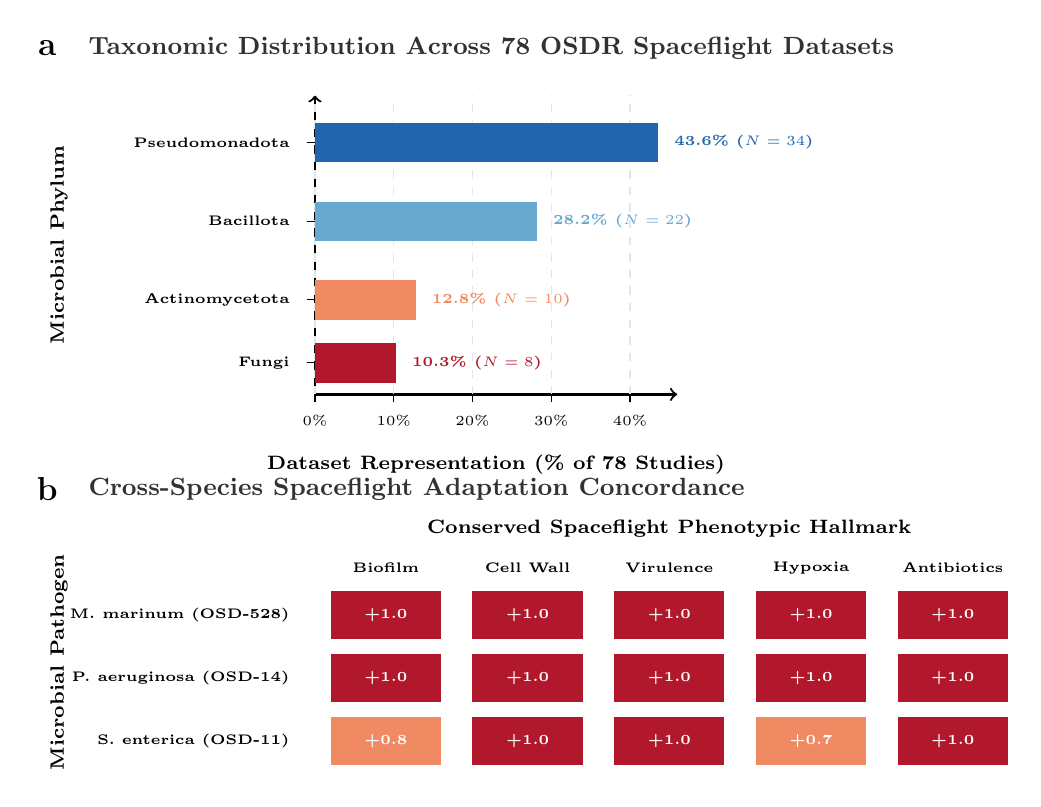
\begin{tikzpicture}[font=\sffamily]
  % Panel a: Taxonomic Distribution with Dedicated Y-axis Clearance (x=3.6 cm)
  \node[font=\large\bfseries] at (0.2, 8.8) {a};
  \node[anchor=west, font=\small\bfseries, text=darkgray] at (0.6, 8.8) {Taxonomic Distribution Across 78 OSDR Spaceflight Datasets};

  % Axes for Panel a: Y-axis placed at x=3.6 cm!
  \draw[->, thick] (3.6, 4.4) -- (3.6, 8.2);
  \node[font=\scriptsize\bfseries, rotate=90] at (0.35, 6.3) {Microbial Phylum};
  \draw[->, thick] (3.6, 4.4) -- (8.2, 4.4) node[midway, below=18pt, font=\scriptsize\bfseries] {Dataset Representation (\% of 78 Studies)};

  % Ticks for Panel a: 3.6 to 7.6 (1.0 cm per 10%)
  \foreach \x/\lbl in {3.6/0\%, 4.6/10\%, 5.6/20\%, 6.6/30\%, 7.6/40\%} {
    \draw (\x, 4.3) -- (\x, 4.4) node[below=4pt, font=\tiny] {\lbl};
    \draw[dashed, draw=gray!20] (\x, 4.4) -- (\x, 8.2);
  }

  % Bars & Y-labels (Labels at x=3.4 anchor=east, bars from x=3.6)
  % 1. Pseudomonadota (43.6% -> x = 3.6 + 0.436*10 = 7.96)
  \draw (3.5, 7.6) -- (3.6, 7.6);
  \node[anchor=east, font=\tiny\bfseries] at (3.4, 7.6) {Pseudomonadota};
  \fill[fairblue] (3.6, 7.35) rectangle (7.96, 7.85);
  \node[anchor=west, font=\tiny\bfseries, text=fairblue] at (8.04, 7.6) {43.6\% ($N=34$)};

  % 2. Bacillota (28.2% -> x = 3.6 + 0.282*10 = 6.42)
  \draw (3.5, 6.6) -- (3.6, 6.6);
  \node[anchor=east, font=\tiny\bfseries] at (3.4, 6.6) {Bacillota};
  \fill[fairmidblue] (3.6, 6.35) rectangle (6.42, 6.85);
  \node[anchor=west, font=\tiny\bfseries, text=fairmidblue] at (6.50, 6.6) {28.2\% ($N=22$)};

  % 3. Actinomycetota (12.8% -> x = 3.6 + 0.128*10 = 4.88)
  \draw (3.5, 5.6) -- (3.6, 5.6);
  \node[anchor=east, font=\tiny\bfseries] at (3.4, 5.6) {Actinomycetota};
  \fill[fairmidred] (3.6, 5.35) rectangle (4.88, 5.85);
  \node[anchor=west, font=\tiny\bfseries, text=fairmidred] at (4.96, 5.6) {12.8\% ($N=10$)};

  % 4. Fungi (10.3% -> x = 3.6 + 0.103*10 = 4.63)
  \draw (3.5, 4.8) -- (3.6, 4.8);
  \node[anchor=east, font=\tiny\bfseries] at (3.4, 4.8) {Fungi};
  \fill[fairred] (3.6, 4.55) rectangle (4.63, 5.05);
  \node[anchor=west, font=\tiny\bfseries, text=fairred] at (4.71, 4.8) {10.3\% ($N=8$)};

  % Panel b: Cross-Species Spaceflight Concordance Heatmap
  \node[font=\large\bfseries] at (0.2, 3.2) {b};
  \node[anchor=west, font=\small\bfseries, text=darkgray] at (0.6, 3.2) {Cross-Species Spaceflight Adaptation Concordance};

  % Axis Titles for Panel b
  \node[font=\scriptsize\bfseries] at (8.1, 2.7) {Conserved Spaceflight Phenotypic Hallmark};
  \node[font=\scriptsize\bfseries, rotate=90] at (0.35, 1.0) {Microbial Pathogen};

  % Column Headers
  \node[font=\tiny\bfseries] at (4.5, 2.2) {Biofilm};
  \node[font=\tiny\bfseries] at (6.3, 2.2) {Cell Wall};
  \node[font=\tiny\bfseries] at (8.1, 2.2) {Virulence};
  \node[font=\tiny\bfseries] at (9.9, 2.2) {Hypoxia};
  \node[font=\tiny\bfseries] at (11.7, 2.2) {Antibiotics};

  % Rows (Labels aligned at x=3.4 anchor=east)
  \node[anchor=east, font=\tiny\bfseries] at (3.4, 1.6) {M. marinum (OSD-528)};
  \fill[fairred] (3.8, 1.3) rectangle (5.2, 1.9); \node[font=\tiny\bfseries, text=white] at (4.5, 1.6) {+1.0};
  \fill[fairred] (5.6, 1.3) rectangle (7.0, 1.9); \node[font=\tiny\bfseries, text=white] at (6.3, 1.6) {+1.0};
  \fill[fairred] (7.4, 1.3) rectangle (8.8, 1.9); \node[font=\tiny\bfseries, text=white] at (8.1, 1.6) {+1.0};
  \fill[fairred] (9.2, 1.3) rectangle (10.6, 1.9); \node[font=\tiny\bfseries, text=white] at (9.9, 1.6) {+1.0};
  \fill[fairred] (11.0, 1.3) rectangle (12.4, 1.9); \node[font=\tiny\bfseries, text=white] at (11.7, 1.6) {+1.0};

  \node[anchor=east, font=\tiny\bfseries] at (3.4, 0.8) {P. aeruginosa (OSD-14)};
  \fill[fairred] (3.8, 0.5) rectangle (5.2, 1.1); \node[font=\tiny\bfseries, text=white] at (4.5, 0.8) {+1.0};
  \fill[fairred] (5.6, 0.5) rectangle (7.0, 1.1); \node[font=\tiny\bfseries, text=white] at (6.3, 0.8) {+1.0};
  \fill[fairred] (7.4, 0.5) rectangle (8.8, 1.1); \node[font=\tiny\bfseries, text=white] at (8.1, 0.8) {+1.0};
  \fill[fairred] (9.2, 0.5) rectangle (10.6, 1.1); \node[font=\tiny\bfseries, text=white] at (9.9, 0.8) {+1.0};
  \fill[fairred] (11.0, 0.5) rectangle (12.4, 1.1); \node[font=\tiny\bfseries, text=white] at (11.7, 0.8) {+1.0};

  \node[anchor=east, font=\tiny\bfseries] at (3.4, 0.0) {S. enterica (OSD-11)};
  \fill[fairmidred] (3.8, -0.3) rectangle (5.2, 0.3); \node[font=\tiny\bfseries, text=white] at (4.5, 0.0) {+0.8};
  \fill[fairred] (5.6, -0.3) rectangle (7.0, 0.3); \node[font=\tiny\bfseries, text=white] at (6.3, 0.0) {+1.0};
  \fill[fairred] (7.4, -0.3) rectangle (8.8, 0.3); \node[font=\tiny\bfseries, text=white] at (8.1, 0.0) {+1.0};
  \fill[fairmidred] (9.2, -0.3) rectangle (10.6, 0.3); \node[font=\tiny\bfseries, text=white] at (9.9, 0.0) {+0.7};
  \fill[fairred] (11.0, -0.3) rectangle (12.4, 0.3); \node[font=\tiny\bfseries, text=white] at (11.7, 0.0) {+1.0};
\end{tikzpicture}
\end{document}
